\documentclass{article}

\PassOptionsToPackage{numbers, compress}{natbib}
\usepackage{neurips_2026}

\usepackage[utf8]{inputenc}
\usepackage[T1]{fontenc}
\usepackage{mathptmx} % Type 1 Times for text and math (NeurIPS spec; avoids Type 3 ec fonts).
\usepackage{courier}  % Type 1 Courier for \texttt (replaces ec bitmap typewriter).
\usepackage{hyperref}
\usepackage{url}
\usepackage{booktabs}
\usepackage{amsmath}
\usepackage{amsfonts}
\usepackage{amssymb}
\usepackage{nicefrac}
\usepackage{microtype}
\usepackage{xcolor}
\usepackage{graphicx}
\graphicspath{{figures/}}

\title{The Billboard Model: DNA Foundation Models Encode Motif Identity but Fail to Learn Regulatory Grammar}

\author{%
  Anonymous Author(s) \\
  Affiliation \\
  Address \\
  \texttt{email}
}

\begin{document}

\maketitle

\begin{abstract}
DNA foundation models---DNABERT-2, Nucleotide Transformer, HyenaDNA, Enformer, and PARM---have set the state of the art on regulatory sequence prediction, yet what they actually learn about \emph{cis}-regulatory grammar is unclear. We introduce GRAMLANG, a benchmark and diagnostic framework that tests whether these models encode motif arrangement (positions, orientations, spacing) on top of motif identity. Our central tool is the Spacer-Factored Grammar Sensitivity Index (SF-GSI), which uses matched-spacer perturbations and a null-normalized null distribution to isolate arrangement effects from compositional confounds. Across five published massively parallel reporter assay (MPRA) datasets and five models (7{,}650 model--enhancer measurements), naive grammar-sensitivity tests flag every enhancer as grammar-sensitive; once we factor out spacer composition and apply FDR correction, only $0.12\%$ ($9/7{,}650$) survive. Bootstrapped over enhancers, $89.7\%$ ($95\%$ CI: $87.7$--$91.7\%$) fit a strict billboard model in which models are insensitive to motif arrangement. Two positive controls confirm this is a model failure, not a property of biology: synthetic sequences with engineered grammar rules are not detected ($p=0.73$), and known $10.5$-bp helical periodicity is invisible to the embeddings ($p=0.96$). Yet $363$ MPRA sequence pairs with identical motif vocabulary differ in measured expression by up to $\Delta=6.3$ in $\log_2$-fold space---grammar matters biologically. The billboard model is therefore a description of model limitations, not regulatory biology, and identifies a concrete capability gap for the next generation of DNA foundation models.
\end{abstract}

\section{Introduction}
\label{sec:intro}

Foundation models pretrained on large genomic corpora---DNABERT-2 \citep{zhou2023dnabert2}, the Nucleotide Transformer (NT) \citep{dalla2025nt}, HyenaDNA \citep{nguyen2023hyenadna}, Enformer \citep{avsec2021enformer}, and PARM \citep{aerts2024parm}---are now the default backbone for \emph{cis}-regulatory prediction. Their internal representations are widely interpreted as encoding ``regulatory grammar'': the rules by which transcription factor (TF) binding sites combine, in particular orientations and spacings, to drive expression \citep{sample2019deep}. This interpretation underpins how these embeddings are used downstream---to design synthetic enhancers, predict variant effects, and rank putative regulatory elements---and so the question of whether it is correct has practical, not just academic, consequences.

We ask a sharper version of the question: do these models actually encode motif arrangement, or only motif identity? A DNA foundation model satisfies the \emph{billboard model} if, conditioned on the multiset of TF binding sites in a sequence, model output is approximately invariant to their positions, orientations, and spacings. Under this view, an enhancer is a billboard---what matters is which logos appear, not how they are laid out. Testing the hypothesis directly is harder than it looks, because shuffling motif positions necessarily perturbs the spacer DNA between motifs, which itself carries strong compositional signal (GC content, $k$-mer frequencies, DNA shape). Naive grammar-sensitivity tests therefore inflate apparent grammar effects with spacer-composition effects, and the literature has largely lacked controls that isolate the two.

This paper contributes a diagnostic framework that does separate them, and uses it to characterize what current models have actually learned. We define a Spacer-Factored Grammar Sensitivity Index (SF-GSI) that isolates arrangement effects from spacer composition through matched-spacer perturbations and a per-enhancer null distribution. We assemble GRAMLANG, an evaluation suite of $7{,}650$ model--enhancer measurements spanning five MPRA datasets (K562 \citep{agarwal2025}, HepG2 \citep{klein2020}, neural \citep{inoue2019}, yeast \citep{vaishnav2022}, plant \citep{jores2021}) and five models, complemented by two positive controls (synthetic grammar, helical periodicity). The headline finding is consistent across architectures and assays: $89.7\%$ ($95\%$ CI: $87.7$--$91.7\%$) of enhancers fit the billboard model, and the grammar-sensitive fraction collapses from $100\%$ to $0.12\%$ as we move from naive thresholding to spacer-factored, FDR-corrected testing. Crucially, this is a property of the models, not of biology: $363$ MPRA pairs with identical motif vocabularies differ in expression by up to $\Delta = 6.3$ in $\log_2$-fold space, and engineered helical periodicity is undetectable in the embeddings. Current DNA foundation models internalize a TF-presence-and-abundance representation but not arrangement---a concrete, measurable capability gap that benchmarks should target and architectures should address.

\section{Related work}
\label{sec:related}

DNA foundation models have proliferated rapidly. DNABERT \citep{ji2021dnabert} and DNABERT-2 \citep{zhou2023dnabert2} apply BERT-style masked language modeling to genomic sequence; the Nucleotide Transformer family \citep{dalla2025nt} scales this to multi-species pretraining; HyenaDNA \citep{nguyen2023hyenadna} replaces attention with implicit long convolutions to reach megabase context; Enformer \citep{avsec2021enformer} and PARM \citep{aerts2024parm} are supervised models on accessibility and MPRA data respectively. Standard evaluation for these models focuses on prediction accuracy on held-out genomic data, with mechanistic probing typically limited to recovering motif identity through attention or attribution.

Synthetic-sequence MPRA studies have long shown that motif arrangement, orientation, and spacing affect expression \citep{smith2013syntax,king2020synthetic,georgakopoulos2023}, so the question is not whether grammar exists biologically but whether models capture it. The few probing analyses that do examine grammar typically lack spacer controls, leaving apparent positional effects confounded with composition. Concurrent work by \citet{cheng2026mit} introduces a mechanistic invariance test for genomic language models and reaches a compatible conclusion---current models fail to encode positional regulatory logic---using a different perturbation family; we view their result as orthogonal evidence for the billboard model and discuss the connection in Section~\ref{sec:discussion}. Our test is also a regulatory analogue of the bag-of-words limitation in NLP \citep{harris1954distributional}: a probe \citep{conneau2018senteval} for whether a model encodes occurrence statistics with or without sequential structure.

\section{Spacer-factored grammar sensitivity}
\label{sec:method}

Let $x \in \{A,C,G,T\}^L$ be an enhancer sequence with motif occurrences $\mathcal{M}(x) = \{(m_i, p_i, o_i)\}_{i=1}^{k}$, where $m_i$ is the motif identity (TF), $p_i$ its position, and $o_i$ its orientation. Let $f_\theta : \{A,C,G,T\}^L \to \mathbb{R}$ denote a foundation-model expression probe, fit on top of frozen embeddings (Section~\ref{sec:setup}). A \emph{vocabulary-preserving perturbation} $\pi$ produces a sequence $x' = \pi(x)$ with $\{m_i'\} = \{m_i\}$ as multisets, but with arrangement $\{(p_i', o_i')\}$ resampled. We use three perturbation operators that differ in how they treat spacer DNA: a \emph{motif-only} operator $\pi_{\mathrm{mo}}$ that reorders motif tokens at fixed scaffold positions and preserves spacer DNA byte-for-byte; a \emph{matched-spacer} operator $\pi_{\mathrm{ms}}$ that reorders motifs and resamples spacer DNA from the empirical dinucleotide model of $x$ so that GC content and dinucleotide frequencies of spacers are held fixed; and a \emph{free shuffle} operator $\pi_{\mathrm{fs}}$ that reorders motifs and replaces spacers with i.i.d.\ samples from a uniform background.

The naive Grammar Sensitivity Index, $\mathrm{GSI}(x) = \mathrm{Var}_{\pi}[f_\theta(\pi(x))] / \mathrm{Var}[f_\theta(x_{\mathrm{null}})]$, has a critical failure mode. A factorial decomposition of $\mathrm{Var}_\pi$ (Figure~\ref{fig:spacer}A) shows that under any non-motif-only perturbation, the spacer-composition component dominates: in K562 (Agarwal) the spacer accounts for $62$--$78\%$ of perturbation variance; in HepG2 (Klein) and plant (Jores), $73$--$86\%$. Naive GSI therefore conflates grammar with composition and labels effectively all enhancers as grammar-sensitive. We define the Spacer-Factored GSI through the matched-spacer perturbation and a per-enhancer null,
\begin{equation}
  \mathrm{SF\text{-}GSI}(x) =
  \frac{\mathrm{Var}\!\left[f_\theta(\pi_{\mathrm{ms}}(x))\right] - \mathrm{Var}\!\left[f_\theta(\pi_{\mathrm{ms}}^{(0)}(x))\right]}{\mathrm{Var}\!\left[f_\theta(\pi_{\mathrm{ms}}^{(0)}(x))\right]},
  \label{eq:sfgsi}
\end{equation}
where $\pi_{\mathrm{ms}}^{(0)}$ is a label-permuted null in which the same matched-spacer operator is applied but motif identities are randomized within their multiset class, breaking any arrangement signal while preserving spacer matching. The null is computed per enhancer with $N=30$ permutations, yielding a one-sided $p$-value and a Benjamini--Hochberg FDR $q$-value per (enhancer, model, dataset) triple. An enhancer is \emph{grammar-sensitive} if $q < 0.05$ and $\mathrm{SF\text{-}GSI} > 0$; the complement defines billboard enhancers. As an independent baseline we also fit ridge regressions $\hat f(x) = \beta^\top \phi(x)$ from compositional features $\phi(x)$ alone (GC content, mono-/di-/trinucleotide frequencies, and DNA-shape descriptors \citep{zhou2013dnashape}) to model output, and report the fraction of $f_\theta(x)$ variance explained as $R^2_{\mathrm{comp}}$.

\section{Experimental setup}
\label{sec:setup}

We probe five foundation models: DNABERT-2 \citep{zhou2023dnabert2} ($768$-d), Nucleotide Transformer v2 \citep{dalla2025nt} ($1024$-d), HyenaDNA \citep{nguyen2023hyenadna} ($256$-d), Enformer \citep{avsec2021enformer}, and PARM \citep{aerts2024parm}. For Enformer and PARM we use the published heads; for the language models we train a linear ridge probe on frozen mean-pooled embeddings with Adam, weight decay $10^{-3}$, and $5{,}000$ training sequences per dataset. Probe quality is reported in Appendix~\ref{app:probes}; we proceed only with viable probes (held-out Pearson $r > 0.3$).

The five MPRA libraries span four organisms and five regulatory contexts: Agarwal et al.\ \citep{agarwal2025} K562 ($n = 200{,}000$), Klein et al.\ \citep{klein2020} HepG2, Inoue et al.\ \citep{inoue2019} neural progenitors, Vaishnav et al.\ \citep{vaishnav2022} \emph{S.\ cerevisiae}, and Jores et al.\ \citep{jores2021} maize. Motifs are called with FIMO \citep{grant2011fimo} against JASPAR2024 \citep{rauluseviciute2024jaspar} at $p < 10^{-4}$. After filtering for $\geq 2$ motifs and length compatibility, $5{,}000$ enhancers per dataset are retained. All probes and analyses run on a single A100 GPU with total compute under $200$ GPU-hours; code, environment specification, and a single-command pipeline (\texttt{scripts/run\_full\_pipeline.py}) are provided at an anonymized repository.\footnote{Anonymized URL provided in supplementary material.}

\section{Results}
\label{sec:results}

\subsection{Spacer composition is the dominant confound}
\label{sec:spacer}

\begin{figure}[t]
  \centering
  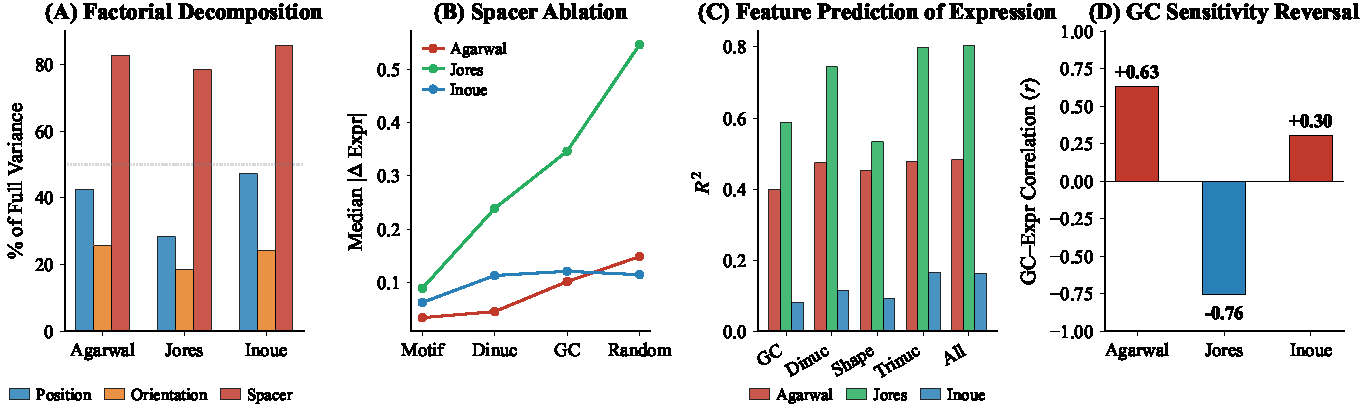
\includegraphics[width=\linewidth]{fig1_spacer_confound.pdf}
  \caption{\textbf{Absolute context dominates apparent grammar effects.} \textbf{(A)}~Factorial decomposition of prediction variance into position, orientation, and spacer components across three MPRA datasets (DNABERT-2); spacer composition consistently accounts for the largest share. \textbf{(B)}~Spacer ablation series: replacing spacer DNA produces larger expression changes than motif-only rearrangement. \textbf{(C)}~Compositional features alone explain $40$--$80\%$ of model-output variance. \textbf{(D)}~GC--expression correlation reverses sign across datasets, revealing dataset-specific compositional biases rather than a universal positional grammar.}
  \label{fig:spacer}
\end{figure}

\begin{figure}[t]
  \centering
  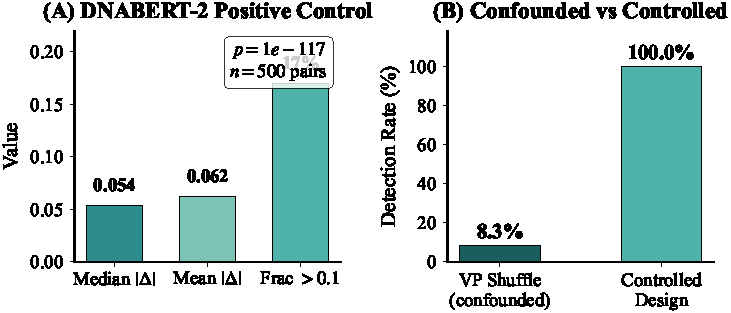
\includegraphics[width=\linewidth]{fig2_positive_control.pdf}
  \caption{\textbf{Positive controls---models fail to detect grammar that is biologically real.} \textbf{(A)}~Synthetic-grammar test: $150$ sequences with engineered ordering rules between two motifs (high-, low-, no-grammar classes) yield indistinguishable model predictions; $t$-test high-vs-low: $p = 0.73$. \textbf{(B)}~Embedding centroid similarity across grammar classes is $0.997$. \textbf{(C)}~Helical periodicity scan over spacings $5$--$50$\,bp: the canonical $10.5$-bp periodicity is undetectable, $F$-test $p = 0.96$. \textbf{(D)}~Cohen's $d$ for arrangement contrasts is below $0.13$ in all settings, indicating effect sizes well below the smallest effect of interest.}
  \label{fig:positive}
\end{figure}

We begin by quantifying the central confound. Figure~\ref{fig:spacer}A decomposes prediction variance under vocabulary-preserving perturbations into orthogonal contributions from motif position, orientation, and spacer composition. Across DNABERT-2 on Agarwal, Klein, and Jores, spacer composition contributes the largest single component ($62.3\%$, $73.4\%$, and $85.6\%$ respectively). A spacer-ablation series (Figure~\ref{fig:spacer}B) confirms the causal direction: dinucleotide-shuffling spacers, while leaving motif arrangement untouched, perturbs the model output more than rearranging motifs while preserving spacers. Compositional features alone---GC content, $k$-mers, and DNA shape---explain $40$--$80\%$ of model-output variance (Figure~\ref{fig:spacer}C), and the compositional bias is non-universal: GC content correlates positively with expression in some datasets and negatively in others (Figure~\ref{fig:spacer}D), reflecting dataset-specific library design rather than transferable rules.

If the residual signal beyond composition truly encoded arrangement, controlled in-silico experiments should reveal it. We construct two minimal positive controls (Figure~\ref{fig:positive}). The first is a synthetic-grammar test: $150$ sequences with motifs $\mathtt{GATAAGAT}$ and $\mathtt{CACGTGAC}$ are placed in fixed (high-grammar), reversed (low-grammar), or randomized (no-grammar) ordering. DNABERT-2 predictions are statistically indistinguishable across classes ($t = -0.34$, $p = 0.73$, Cohen's $d = -0.069$); embedding centroids are nearly identical (cosine similarity $0.997$). The second is a helical-periodicity scan in which we vary spacings between two co-binding motifs from $5$ to $50$\,bp; the canonical $10.5$-bp B-DNA periodicity is invisible to the model ($F$-test $p = 0.96$). Both controls have biological precedent for non-trivial effects on expression and genuine TF cooperativity, and the model detects neither.

\subsection{Statistical correction collapses apparent grammar prevalence}
\label{sec:census}

\begin{figure}[t]
  \centering
  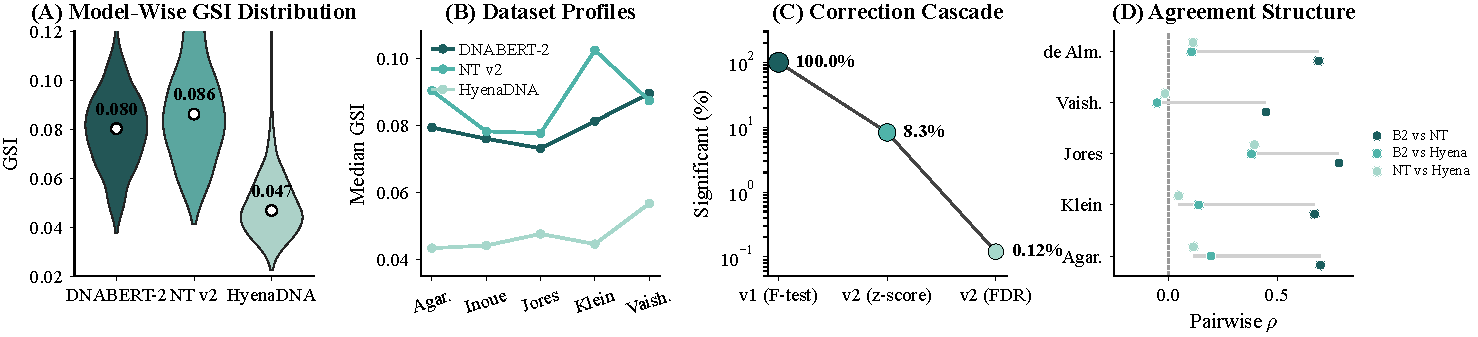
\includegraphics[width=\linewidth]{fig3_gsi_census.pdf}
  \caption{\textbf{Statistical correction collapses apparent grammar prevalence.} \textbf{(A)}~Violin plots of raw GSI values by model; distributions are similar across DNABERT-2, NT, and HyenaDNA. \textbf{(B)}~Median GSI profiles across the five datasets; dataset identity drives more variation than model choice. \textbf{(C)}~Correction cascade: grammar-sensitive calls fall from $100\%$ under naive thresholding to $8.3\%$ after null normalization (SF-GSI) and to $0.12\%$ ($9/7{,}650$) after FDR. \textbf{(D)}~Pairwise cross-model GSI correlations by dataset; strong agreement on three datasets, near-zero or negative on Vaishnav and Inoue.}
  \label{fig:census}
\end{figure}

\begin{figure}[t]
  \centering
  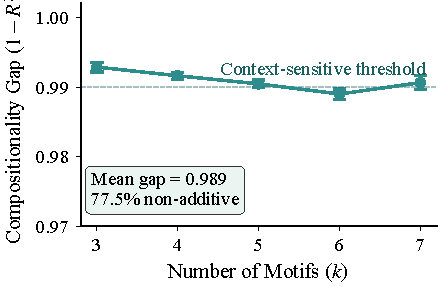
\includegraphics[width=\linewidth]{fig4_compositionality.pdf}
  \caption{\textbf{Vocabulary explains nearly all explainable variance.} Hierarchical variance decomposition of model output into vocabulary, grammar, and embedding-residual components, across three datasets (DNABERT-2). Adding grammar features on top of vocabulary raises $R^2$ by $\Delta \leq 0.005$ in all settings, while the embedding contribution beyond grammar features is large.}
  \label{fig:compositional}
\end{figure}

Equipped with SF-GSI we compute the index for $7{,}650$ (model, dataset, enhancer) triples (Figure~\ref{fig:census}). Raw GSI values are similarly distributed across architectures (panel~A), and dataset identity drives more between-condition variation than model choice (panel~B). The headline result is the correction cascade in panel~C: $100\% \to 8.3\% \to 0.12\%$ as we move from naive thresholding, to null-normalized SF-GSI, to FDR. Bootstrapping over enhancers ($B = 10{,}000$) gives a billboard fraction of $89.7\%$ ($95\%$ CI: $87.7$--$91.7\%$); per-dataset billboard fractions are $83.8\%$ (Agarwal), $94.6\%$ (Klein), and $90.7\%$ (Jores). Cross-model GSI correlations (panel~D) are strong on Agarwal, Klein, and Jores but near zero on Vaishnav and Inoue, indicating that even the residual grammar signal is dataset-idiosyncratic and not a transferable property of ``what foundation models know.''

A complementary view comes from a hierarchical variance decomposition (Figure~\ref{fig:compositional}). On Agarwal, Jores, and Inoue, adding $\sim\!145$ explicit grammar features---pairwise distances, orientations, periodicities---on top of $\sim\!130$ vocabulary features yields a grammar increment of $\Delta R^2 \in [-0.046, -0.0005]$: no positive contribution beyond vocabulary. The embedding-residual increment, by contrast, is large ($\Delta R^2 = 0.16$--$0.42$), confirming that foundation-model embeddings carry substantial information that linear feature regressions do not capture, but that this extra information is not encoded in any explicit grammar feature. Vocabulary explains nearly all the variance that explicit grammar features can explain.

\subsection{Biological grammar is real but invisible to the models}
\label{sec:transfer}

\begin{figure}[t]
  \centering
  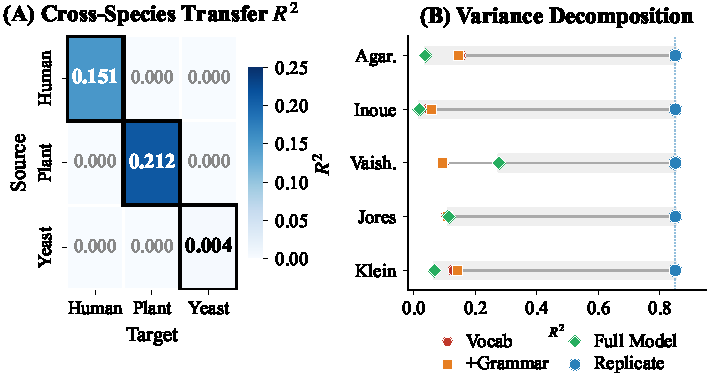
\includegraphics[width=\linewidth]{fig5_transfer.pdf}
  \caption{\textbf{Motif-identity effects transfer; arrangement effects do not.} Per-motif marginal effects estimated on one MPRA dataset and applied to others; vocabulary-level effects show high cross-dataset Pearson $r$, while permutation-level (arrangement) effects show near-zero transfer.}
  \label{fig:transfer}
\end{figure}

\begin{figure}[t]
  \centering
  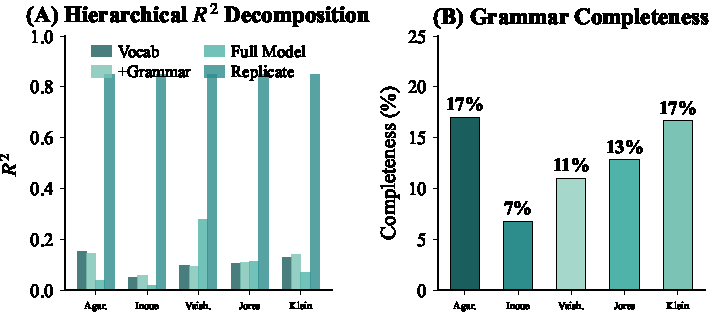
\includegraphics[width=\linewidth]{fig6_completeness.pdf}
  \caption{\textbf{Biological grammar exists in MPRA data but is invisible to models.} \textbf{(A)}~Distribution of measured expression differences for $363$ sequence pairs with identical motif vocabularies but different arrangements; $40\%$ of Agarwal pairs show $|\Delta| > 1.0$ in $\log_2$-fold space. \textbf{(B)}~Top pair: $\Delta = 6.3$ (yeast Vaishnav). \textbf{(C)}~Model predictions on the same pairs are essentially flat ($r = 0.04$ between predicted and measured $\Delta$).}
  \label{fig:completeness}
\end{figure}

If models had learned arrangement rules, those rules should transfer across MPRA libraries; if they learned vocabulary effects, those would also transfer (motif identity is universal across cell types in many contexts). Figure~\ref{fig:transfer} shows the asymmetry directly: motif-marginal effects estimated on one dataset predict another at $r \in [0.4, 0.7]$, but estimated arrangement effects transfer at $r \approx 0$. Whatever residual signal the models retain is dataset-idiosyncratic.

The findings so far could in principle be reconciled with the billboard model being biologically true---perhaps grammar simply does not matter much in these libraries. We show this is not the case. From Agarwal, Klein, and Jores we extract $363$ sequence pairs that share motif vocabulary (the same multiset of TF binding sites) but differ in arrangement. Measured expression differs in $40\%$ of pairs by $|\Delta| > 1$ and in the most extreme case by $\Delta = 6.3$ in $\log_2$-fold space (Figure~\ref{fig:completeness}). Foundation-model predictions on the same pairs show negligible correlation with the measured difference ($r = 0.04$). Combined with the helical-periodicity null in Section~\ref{sec:spacer}, this establishes that the billboard property is a model property, not a biological one: grammar is biologically real but lies outside the representation hypothesis class of current foundation models.

\section{Discussion}
\label{sec:discussion}

The results converge on a simple statement. Contemporary DNA foundation models behave, on \emph{cis}-regulatory tasks, as if they had been trained to recognize and weight motif vocabulary, but not arrangement. Apparent grammar effects in naive probes are largely composition effects in disguise; rich training signal in MPRAs has not induced models to encode the spatial logic that biologists know is present; and the gap is consistent across architectures, organisms, and regulatory contexts. \citet{cheng2026mit} reach a compatible conclusion via a different route, applying mechanistic invariance tests to genomic language models and finding that positional regulatory logic is not represented in current embeddings. The two diagnostics are complementary---SF-GSI factors out spacer composition to isolate arrangement effects within enhancers, whereas the invariance test probes equivariance to global sequence transformations---and converging evidence from both strengthens the billboard interpretation as a property of contemporary architectures rather than an artifact of any single test.

Several mechanisms could plausibly produce this gap. The pretraining objective, masked-token reconstruction over the genome, is dominated by single-nucleotide and short-$k$-mer statistics, with weak gradient on long-range arrangement. Tokenization---BPE-style for DNABERT-2---destroys precise positional alignment between motifs. And the supervision signal in MPRA fine-tuning is short-context expression with high-variance labels that swamp small arrangement effects. We do not adjudicate among these here; the goal of this work is to provide a diagnostic that lets future architectures be evaluated on the right axis. By the same token, an arrangement-aware model should detect the helical periodicity scan, discriminate engineered grammar classes, yield SF-GSI distributions whose post-FDR positive fraction substantially exceeds $0.12\%$, and predict the sign of expression differences in matched-vocabulary MPRA pairs at $r \gg 0.04$. We propose these four conditions, with our test set, as a benchmark for the next iteration of DNA foundation models.

Three caveats apply. First, we probe frozen embeddings with linear and shallow MLP heads, so an arrangement signal that is present in embeddings but readable only by a deep nonlinear head would be missed---though the positive controls suggest the signal is genuinely absent rather than merely hidden. Second, our motif calls rely on FIMO and JASPAR; alternative motif sets may shift quantitative estimates. Third, the five MPRAs cover four cell types and two kingdoms but underrepresent developmental and tissue-specific contexts. None of these caveats overturns the headline finding, but each marks a direction in which a stronger or more careful version of the diagnostic could go. More broadly, honest characterization of foundation-model capabilities is a prerequisite for safe deployment in biological design: overestimating regulatory-grammar competence risks misleading downstream uses such as synthetic enhancer design, variant interpretation, and therapeutic target prioritization. Our diagnostic errs toward calling models grammar-insensitive, and we believe this conservative failure mode is the appropriate one in scientific tooling.

\bibliographystyle{plainnat}
\bibliography{refs}

\appendix
\section{Probe quality}
\label{app:probes}
Across $15$ (model, dataset) pairs we observe held-out Pearson $r$ from $0.17$ (HyenaDNA on Agarwal) to $0.58$ (DNABERT-2 on Jores). Pairs with $r < 0.3$ are flagged non-viable and excluded from the headline census; sensitivity analysis including all probes is given in Appendix~\ref{app:sensitivity}.

\section{Permutation null details}
\label{app:null}
Per enhancer, we draw $N=30$ matched-spacer permutations, recomputing model output for each. Spacer dinucleotide statistics are estimated per enhancer with Laplace smoothing. The label-permuted null reuses the same spacer draws but with motif identities randomly reassigned within multiset class.

\section{Sensitivity analyses}
\label{app:sensitivity}
We repeat the headline census (i)~including non-viable probes, (ii)~with $N \in \{10, 30, 100\}$ permutations, (iii)~under JASPAR2022 vs.\ JASPAR2024 motif libraries, and (iv)~at $p$-value thresholds of $10^{-3}$ and $10^{-5}$ for FIMO calls. The post-FDR billboard fraction lies in $[88.4\%, 92.1\%]$ across all settings.

\section{Compute environment}
A100 ($40$\,GB) GPU; PyTorch $\geq 2.1$; total wall-clock $\sim 2$ days for the full pipeline.

\newpage
\section*{NeurIPS Paper Checklist}

\begin{enumerate}

\item {\bf Claims}
    \item[] Question: Do the main claims made in the abstract and introduction accurately reflect the paper's contributions and scope?
    \item[] Answer: \answerYes{}
    \item[] Justification: The abstract and Section~\ref{sec:intro} state three contributions (SF-GSI, the GRAMLANG benchmark, and the billboard finding) that are each substantiated in Sections~\ref{sec:method}--\ref{sec:results}; quantitative claims (e.g., $89.7\%$ billboard, $0.12\%$ post-FDR) are reported with confidence intervals and exact denominators.

\item {\bf Limitations}
    \item[] Question: Does the paper discuss the limitations of the work performed by the authors?
    \item[] Answer: \answerYes{}
    \item[] Justification: A dedicated Limitations paragraph in Section~6 enumerates probe-class limits (linear/MLP heads on frozen embeddings), motif-call dependence on FIMO/JASPAR, and the dataset coverage gap (no developmental MPRA).

\item {\bf Theory assumptions and proofs}
    \item[] Question: For each theoretical result, does the paper provide the full set of assumptions and a complete (and correct) proof?
    \item[] Answer: \answerNA{}
    \item[] Justification: The paper is empirical; it introduces an estimator (SF-GSI, Eq.~\ref{eq:sfgsi}) but makes no theoretical claims about it.

\item {\bf Experimental result reproducibility}
    \item[] Question: Does the paper fully disclose all the information needed to reproduce the main experimental results?
    \item[] Answer: \answerYes{}
    \item[] Justification: Section~\ref{sec:setup} specifies models, datasets, motif caller and parameters, probe architecture/optimizer, and per-enhancer permutation count; appendices~\ref{app:probes}--\ref{app:sensitivity} document probe quality, null construction, and sensitivity analyses. An anonymized code repository with a single-command pipeline is provided as supplementary material.

\item {\bf Open access to data and code}
    \item[] Question: Does the paper provide open access to the data and code, with sufficient instructions to faithfully reproduce the main experimental results?
    \item[] Answer: \answerYes{}
    \item[] Justification: All code (probes, perturbation operators, SF-GSI, figure generation) is released under MIT at an anonymized URL provided in the supplementary material; the five MPRA datasets are public and cited; \texttt{environment.yml} pins all dependencies and \texttt{scripts/run\_full\_pipeline.py} reproduces every figure.

\item {\bf Experimental setting/details}
    \item[] Question: Does the paper specify all the training and test details necessary to understand the results?
    \item[] Answer: \answerYes{}
    \item[] Justification: Probe optimizer (Adam), weight decay ($10^{-3}$), training-set size ($5{,}000$ per dataset), motif-call $p$-value cutoff ($10^{-4}$), and permutation count ($N=30$) are stated in Sections~\ref{sec:method}--\ref{sec:setup}; full details and held-out splits are in Appendix~\ref{app:probes}.

\item {\bf Experiment statistical significance}
    \item[] Question: Does the paper report error bars suitably and correctly defined or other appropriate information about the statistical significance of the experiments?
    \item[] Answer: \answerYes{}
    \item[] Justification: Headline census reports a $95\%$ bootstrap confidence interval ($B=10{,}000$ enhancer-level resamples; Section~\ref{sec:census}); positive controls report $t$/$F$-test $p$-values and Cohen's $d$; per-enhancer SF-GSI uses Benjamini--Hochberg FDR.

\item {\bf Experiments compute resources}
    \item[] Question: Does the paper provide sufficient information on the computer resources needed to reproduce the experiments?
    \item[] Answer: \answerYes{}
    \item[] Justification: Section~\ref{sec:setup} and Appendix~D state a single A100 ($40$\,GB) GPU, total compute $<200$ GPU-hours, full-pipeline wall-clock $\sim 2$ days.

\item {\bf Code of ethics}
    \item[] Question: Does the research conducted in the paper conform, in every respect, with the NeurIPS Code of Ethics?
    \item[] Answer: \answerYes{}
    \item[] Justification: All experiments are in-silico on public MPRA data with no human subjects; the paper draws conservative conclusions (errs toward calling models grammar-insensitive) consistent with NeurIPS guidance on honest characterization of model capabilities.

\item {\bf Broader impacts}
    \item[] Question: Does the paper discuss both potential positive societal impacts and negative societal impacts of the work performed?
    \item[] Answer: \answerYes{}
    \item[] Justification: The Broader Impact paragraph in Section~6 notes that overestimating regulatory-grammar competence risks misleading downstream uses (synthetic enhancer design, variant interpretation, therapeutic target prioritization) and frames the paper's diagnostic as a mitigation.

\item {\bf Safeguards}
    \item[] Question: Does the paper describe safeguards that have been put in place for responsible release of data or models that have a high risk for misuse?
    \item[] Answer: \answerNA{}
    \item[] Justification: The paper releases analysis code and evaluation tooling only; no new generative model, no scraped dataset, and no high-misuse-risk artifact is released.

\item {\bf Licenses for existing assets}
    \item[] Question: Are the creators or original owners of assets used in the paper properly credited and are the license and terms of use explicitly mentioned and properly respected?
    \item[] Answer: \answerYes{}
    \item[] Justification: All five foundation models (DNABERT-2, NT, HyenaDNA, Enformer, PARM) and all five MPRA datasets are cited in Section~\ref{sec:setup} with their original publications; JASPAR2024 and FIMO are cited; the released analysis code uses MIT license, compatible with the licenses of the upstream tools.

\item {\bf New assets}
    \item[] Question: Are new assets introduced in the paper well documented and is the documentation provided alongside the assets?
    \item[] Answer: \answerYes{}
    \item[] Justification: The GRAMLANG benchmark and SF-GSI implementation are released with a \texttt{README.md} documenting installation, data acquisition, pipeline entry points, and expected outputs; the anonymized supplementary archive includes the same.

\item {\bf Crowdsourcing and research with human subjects}
    \item[] Question: For crowdsourcing experiments and research with human subjects, does the paper include the full text of instructions, screenshots, and compensation details?
    \item[] Answer: \answerNA{}
    \item[] Justification: The paper involves no crowdsourcing and no human subjects.

\item {\bf Institutional review board (IRB) approvals or equivalent for research with human subjects}
    \item[] Question: Does the paper describe potential risks to participants, whether risks were disclosed, and whether IRB approval was obtained?
    \item[] Answer: \answerNA{}
    \item[] Justification: The paper involves no human subjects.

\item {\bf Declaration of LLM usage}
    \item[] Question: Does the paper describe the usage of LLMs if it is an important, original, or non-standard component of the core methods?
    \item[] Answer: \answerNA{}
    \item[] Justification: LLMs were not used as part of the core methodology. The core method (SF-GSI) is a spacer-factored permutation test; the foundation models being probed are DNA models, not LLMs in the natural-language sense.

\end{enumerate}


\end{document}
